%=============================================================================
% Domain-Aware Federated Log Anomaly Detection under Heterogeneous and
% Sequentially Arriving Domains
%
% Target venue: IEEE Access.
% This source compiles with a standard TeX install (IEEEtran journal class).
% To switch to the official IEEE Access template, replace the \documentclass and
% preamble with ieeeaccess.cls (available from the IEEE Author Center); the body,
% tables, figures, and \cite/\bibliography commands below carry over unchanged.
%
% HARD RULE: every numeric result traces to a CSV in ../../results/ (see
% docs/paper/HANDOFF.md and docs/RESEARCH_LOG.md for provenance). Do NOT invent numbers.
%=============================================================================
\documentclass[journal]{IEEEtran}

\usepackage{graphicx}
\usepackage{booktabs}
\usepackage{amsmath}
\usepackage{amssymb}
\usepackage{url}
\usepackage[hidelinks]{hyperref}
\graphicspath{{../../results/}}

\begin{document}

\title{Domain-Aware Federated Log Anomaly Detection under Heterogeneous and
Sequentially Arriving Domains}

\author{Vansh~Mundhra,~Pinak~Debnath,~and~Sankari~M% <-this % stops a space
\thanks{The authors are with the School of Computer Science and Engineering,
Vellore Institute of Technology (VIT), Chennai, India
(e-mail: vansh.mundhra@example.edu; pinak.debnath@example.edu; sankari.m@vit.ac.in).}%
\thanks{Manuscript prepared July 2026. Corresponding author: V.~Mundhra.}}

\markboth{Preprint --- submitted to IEEE Access}%
{Mundhra \MakeLowercase{\textit{et al.}}: Domain-Aware Federated Log Anomaly Detection}

\maketitle

\begin{abstract}
Federated log anomaly detection has recently been reported to have two attractive
properties: lightweight statistical detectors are approximately \emph{invariant to client
data distribution}, and their model size is \emph{bounded by a finite event vocabulary}.
These properties, however, were established only in a \emph{homogeneous} setting, where every
federated client holds a slice of the \emph{same} log dataset (quantity skew). We ask whether
they survive a \emph{heterogeneous} federation (clients from different log domains) and an
\emph{evolving} one (new domains arriving over time). Using the HDFS and BGL benchmarks over a
single merged 427-event vocabulary, we show that (H1) domain-blind range-based aggregation
collapses on the tighter-distributed domain (HDFS Length $F_1$ falls from a single-domain
$0.538$ to $0.000\pm0.000$ across five seeds), and that a simple \emph{domain-aware}
aggregation restores it to $0.561\pm0.024$, i.e., back to its single-domain value, while
leaving the other domain untouched. For deep models we find a sharper distinction than prior
work anticipates: \emph{simultaneous} mixed Federated Averaging does \emph{not} degrade (H2),
even under a learned embedding input, whereas \emph{sequential} arrival of a new domain
\emph{catastrophically forgets} the earlier one (H3: HDFS $F_1$ $0.70\!\rightarrow\!0.04$,
forgetting $0.665\pm0.003$ over three seeds)---but only when the input representation makes the
two vocabularies share a feature space. A controlled experiment (scalar identifier versus
learned embedding) isolates this cause. Set-union detectors, separately, never forget but grow
$\times3.7$ as a single domain arrives, breaking the bounded-size property under evolution. The
result is a precise $2\times2$ map---\{simultaneous, sequential\}$\times$\{disjoint, shared
representation\}, in which exactly one cell fails; we further show this failure is \emph{directional},
occurring only when a broad-vocabulary domain is onboarded after a narrow one. We give working fixes
for both failures: a domain-aware aggregation that restores the collapsed range method (routing with no
oracle domain tag, at $100\%$ inferred-routing accuracy), and, for the forgetting, both a small replay
buffer ($\approx10\%$ of the earlier domain's data, cutting forgetting from $0.665$ to $0.004$) and a
memory-free EWC alternative, which we compare directly. All results are reproduced from real runs on
commodity CPU.
\end{abstract}

\begin{IEEEkeywords}
Federated learning, log anomaly detection, data heterogeneity, domain skew, catastrophic
forgetting, continual learning, DeepLog, model aggregation.
\end{IEEEkeywords}

\section{Introduction}
\IEEEPARstart{S}{ystem} logs are the primary forensic record of large software and
infrastructure deployments, and detecting anomalous log sequences is central to reliability,
availability, and security engineering~\cite{he2016experience,landauer2023survey}. As logs
increasingly originate from distributed, privacy-sensitive, or bandwidth-constrained sources
(IoT fleets, industrial networks, smart grids, multi-tenant clouds), centralizing them for
analysis is often infeasible. Federated learning~\cite{mcmahan2017communication} offers an
alternative: clients train locally and share only model updates, keeping raw logs on premises.

A recent, careful study by Pustozerova \emph{et al.}~\cite{pustozerova2026lightweight}
benchmarks \emph{lightweight statistical} detectors (sequence-length ranges, sets of seen
events, count-vector nearest neighbours) against \emph{deep} detectors
(DeepLog~\cite{du2017deeplog}, LogAnomaly~\cite{meng2019loganomaly}) under Federated
Averaging (FedAvg). They report two encouraging properties: (C1) lightweight detectors are
approximately \emph{invariant to client data distribution}, so their federated $F_1$ matches the
centralized value even under non-IID splits; and (C2) their model size is \emph{bounded by a
finite event vocabulary}, so once the vocabulary saturates, memory stabilizes.

\textbf{The gap.} That evaluation is \emph{homogeneous}. Their non-IID setting is
\emph{quantity skew}: each client receives a different \emph{amount} of training data, drawn by a
log-normal allocation, but every client still holds a slice of the \emph{same} dataset (HDFS
\emph{or} BGL, never both). Real federations are \emph{domain-heterogeneous} (different services,
systems, and vendors produce categorically different logs) and \emph{evolving}, onboarding new
log sources over time. This is precisely the regime the two claims were never tested in; indeed
the public artifact of~\cite{pustozerova2026lightweight} ships \texttt{hdfs\_*} and \texttt{bgl\_*}
configurations but no mixed configuration.

\textbf{This paper.} We place HDFS and BGL clients in \emph{one} federation over a merged event
vocabulary, and separately let domains arrive \emph{sequentially}, and we test C1 and C2 directly.
Our findings form a compact map of when federated log anomaly detection is safe and when it is
not, and why. Concretely:

\begin{itemize}
\item \textbf{H1 (range aggregation).} Domain-blind range aggregation \emph{collapses} on the
tighter-distributed domain: BGL's large length spread widens the shared global range until almost
no HDFS anomaly is flagged, driving HDFS Length $F_1$ from $0.538$ to $0.000$. A simple
\emph{domain-aware} aggregation (keep per-domain range parameters and route by a domain tag) restores
HDFS to $0.561$, its single-domain level, without touching BGL. The failure is a clean
counterexample to C1 under domain skew.
\item \textbf{H2 (simultaneous mixing).} FedAvg on DeepLog does \emph{not} degrade when HDFS and
BGL clients train together; it even improves BGL. This holds under both a scalar-identifier input
and a learned embedding, and thus \emph{strengthens} the deep model's generality claim.
\item \textbf{H3 (sequential arrival) and the mechanism.} When a new domain instead arrives
\emph{sequentially}, the deep model \emph{catastrophically forgets} the earlier one
($F_1$ $0.70\!\rightarrow\!0.04$)---but only when the input representation forces the two
vocabularies to share a feature space. A controlled scalar-vs-embedding experiment isolates
representation, not the aggregation method, as the cause. Set-union detectors never forget but
grow $\times3.7$ per added domain, breaking C2 under evolution.
\end{itemize}

Our contributions are: (i) a merged cross-domain vocabulary and dataloader that let heterogeneous
log clients share one federation---the enabling artifact absent from prior pipelines; (ii) to our knowledge, the
first empirical demonstration, across five seeds and both IID and non-IID splits, that domain-blind
range aggregation fails under domain skew, with a minimal domain-aware fix that restores single-domain
performance and routes at inference with no oracle tag ($100\%$ inferred-routing accuracy);
(iii) a controlled analysis showing that \emph{simultaneous} mixing is safe but \emph{sequential}
arrival is catastrophic \emph{iff} the representation shares a feature space, and that this forgetting is
\emph{directional} (only broad-after-narrow onboarding forgets), together with two mitigations we compare
head-to-head---a memory-based replay buffer and memory-free EWC---that each remove the forgetting; and
(iv) a reproducible, CPU-only artifact
in which every reported number traces to a result file.

\section{Related Work}

\subsection{Log anomaly detection}
Log-based anomaly detection typically parses raw lines into event templates (most commonly with
Drain~\cite{he2017drain}) and then classifies template sequences. Classical detectors use
statistical features such as event-count vectors, PCA projections, or invariants; deep detectors
model sequences directly. DeepLog~\cite{du2017deeplog} trains an LSTM to predict the next event
from a sliding window and flags a sequence when the true next event is not among the model's
top-$g$ predictions. LogAnomaly~\cite{meng2019loganomaly} extends this with template semantics and
quantitative patterns. Surveys~\cite{landauer2023survey} and empirical
studies~\cite{he2016experience} report that no single method dominates across datasets, motivating
the ensemble baselines we also study. We reuse the DeepLog mechanism and the HDFS/BGL benchmarks
from Loghub~\cite{zhu2023loghub}, but ask a question orthogonal to detector design: what happens
when clients hold \emph{different} log domains.

\subsection{Federated learning and data heterogeneity}
FedAvg~\cite{mcmahan2017communication} aggregates client models by weighted parameter averaging.
Data heterogeneity is the central obstacle: Zhao \emph{et al.}~\cite{zhao2018federated} show that
label skew induces weight divergence and can cut accuracy by tens of points, and the field survey
of Kairouz \emph{et al.}~\cite{kairouz2021advances} catalogues quantity, label, and feature skew as
distinct regimes. The heterogeneity we study---\emph{domain} skew, where clients hold data from
different generative processes with largely disjoint vocabularies---sits at the extreme of feature
skew and is comparatively under-explored for log data. Notably, our H2 result is a partial
counterpoint to the usual ``non-IID hurts FedAvg'' narrative: for a next-event LSTM with a
scalar-identifier input, simultaneous domain mixing does \emph{not} degrade accuracy, because the
domains occupy disjoint input ranges and never actually compete for the same parameters. We show
this robustness is representation-dependent, which reconciles the two narratives.

\subsection{Federated log anomaly detection}
The closest work is Pustozerova \emph{et al.}~\cite{pustozerova2026lightweight}, whose lightweight
methods, datasets, and FedAvg pipeline we adopt, and whose two claims (C1, C2) we test outside
their homogeneous setting. A companion line of work studies federated \emph{deep} log detection and
its open challenges~\cite{fedlog2024openchallenges}. Most recently, FedLAD~\cite{fedlad2025}
provides a modular testbed for federated log anomaly detection across client configurations. These
efforts either (a) keep every client on the same dataset (quantity/label skew) or (b) provide
infrastructure to vary clients, but none isolates the two published invariance/bounded-size claims
under a \emph{single federation that mixes two distinct log domains} or under \emph{sequential
domain arrival}, and none identifies the input representation as the variable governing forgetting.
That specific gap is our target.

\subsection{Continual and federated continual learning}
Sequential domain arrival is a continual-learning problem. Catastrophic forgetting---the loss of
earlier-task performance after training on a new task---is a long-standing phenomenon, and elastic
weight consolidation (EWC)~\cite{kirkpatrick2017overcoming} and the broader continual-learning
literature~\cite{delange2022continual} propose mitigations. When continual learning is combined
with federation, forgetting compounds with non-IID aggregation~\cite{cfl2023quantifying}. Our H3
result contributes a concrete, reproducible instance in the log-analytics domain and, crucially,
shows that whether forgetting occurs at all is decided by the input representation---a lever
orthogonal to EWC-style penalties, which we flag as complementary future work.

\subsection{Count-vector detectors}
One ensemble member, ECVC, scores a sequence by the distance of its normalized event-count
histogram to the nearest normal histogram~\cite{ecvc2024}. We reimplement this method from its
published description to study whether repairing the range component lifts the full ensemble.

\section{Problem Setting}
We consider a federation of $K$ clients, each holding semi-supervised training data (normal
sequences only) drawn from one \emph{domain} $d\in\mathcal{D}$. Each domain has its own event
template set; a global model is formed by aggregating client models. We test two published claims
of~\cite{pustozerova2026lightweight}:
\begin{itemize}
\item \textbf{C1 (distribution invariance).} For lightweight detectors built by deterministic
set-union or min--max aggregation, the global model is ``independent of client data
distributions,'' so federated $F_1$ equals the centralized $F_1$.
\item \textbf{C2 (bounded growth).} Model size is bounded by the finite event vocabulary; once the
vocabulary saturates, memory stabilizes.
\end{itemize}
Both were validated only under \emph{quantity skew within one dataset}. We evaluate them under
\emph{domain skew} (Sections~\ref{sec:h1},~\ref{sec:h2}) and \emph{sequential domain arrival}
(Section~\ref{sec:h3}).

\section{Method}

\subsection{Merged cross-domain vocabulary}
To let heterogeneous clients share one federation we build a single global event space. Each
domain's parsed templates form a contiguous identifier block: HDFS occupies global ids $[0,33)$ and
BGL $[33,427)$, so the merged vocabulary has $427$ events. A \texttt{domain} tag travels with every
sequence, enabling per-domain evaluation and domain-aware routing. HDFS and BGL both reuse small
integers for \emph{different} templates; we therefore key each event as
\texttt{domain:id}, so that HDFS ``5'' maps to global id $0$ while BGL ``5'' maps to global id
$43$, and the two never collide. This mirrors the reference pipeline's per-dataset global dictionary,
extended across datasets.

\subsection{Federation construction}
Each domain contributes $N_d$ clients. Following the reference convention, $1\%$ of each domain's
normal sequences form the training pool (the remainder is held out for evaluation), partitioned
across that domain's clients either uniformly (IID) or by a log-normal quantity skew
($\sigma=0.25$) matching the reference non-IID setting. Unless stated otherwise, the mixed
federation is 3 HDFS + 2 BGL clients over the merged $427$-event vocabulary.

\subsection{Detectors}
\emph{Length} learns the $[\min,\max]$ length of normal sequences and flags anything outside;
domain-blind FedAvg takes the global min-of-mins and max-of-maxes. \emph{Known Events} learns the
set of normal event ids (FedAvg is set union) and flags any unseen event. \emph{ECVC} scores a
sequence by the $L_1$ distance of its normalized event-count histogram to the nearest normal
histogram, with a supervised threshold. \emph{DeepLog}~\cite{du2017deeplog} is a two-layer,
64-unit LSTM predicting the next event from a length-10 window; a sequence is anomalous if the true
next event is not among the top-9 predictions, and FedAvg averages client weights. To study
representation effects we support two DeepLog input encodings: the reference's raw scalar event id
(input size 1), and a learned 16-dimensional embedding.

\subsection{Domain-aware aggregation (the fix)}\label{sec:da}
Instead of one global range, domain-aware Length keeps a \emph{per-domain} $[\min,\max]$, aggregated
only across clients of the same domain, and routes a test sequence to its domain's range using the
domain tag. This preserves the federation (clients of a domain still collaborate) while removing
the cross-domain contamination that causes H1. Because a domain's aggregated range is the min--max
over the union of that domain's client data, it is \emph{invariant} to how the data is partitioned
across clients, so the fix is robust to quantity skew by construction.

\textbf{Removing the oracle tag.} The routing above assumes a domain tag on each test sequence.
A real deployment may not provide one, so we consider two tag-free strategies. \emph{Vocabulary-block
routing} infers a sequence's domain from its event ids: because each domain owns a contiguous, disjoint
id block ($[0,33)$ for HDFS, $[33,427)$ for BGL), a sequence's domain is the majority block of its ids,
and a sequence with an id outside every block is flagged as anomalous (unknown domain). \emph{Conservative
routing} avoids inference entirely, flagging a sequence only if its length is outside \emph{every}
domain's range. We evaluate both against the oracle in Section~\ref{sec:h1}: vocabulary-block routing
reproduces the oracle-tag $F_1$ exactly (so the fix is deployable without any external domain label),
whereas conservative routing collapses on the tighter domain.

\section{Experimental Setup}\label{sec:setup}
We use the HDFS and BGL benchmarks from Loghub~\cite{zhu2023loghub}, parsed into event-id sequences.
HDFS has 33 event types, $558{,}223$ normal and $16{,}838$ abnormal sequences (average length
$29\pm6$); BGL has 394 event types, $37{,}823$ normal and $31{,}429$ abnormal sequences (average
length $69\pm747$). The merged vocabulary is $427$. We report per-domain precision, recall, and
$F_1$ (anomaly is the positive class), forgetting ($F_1^{\text{before}}-F_1^{\text{after}}$), and
model state size in bytes. Seeds $0$--$4$ are used where noted, and we report mean $\pm$ population
standard deviation. All experiments run on commodity CPU; DeepLog evaluation is made tractable by
deduplicating identical test sequences and weighting by count.

Before any mixed-domain conclusion, we reproduce single-domain baselines
(Table~\ref{tab:repro}). Our numbers match the reference picture: HDFS Length is weak alone
($0.538$ vs.\ their $\sim$0.57), BGL Known Events is strong ($0.992$ vs.\ their $\sim$0.99), and the
right methods are strong/weak on the right datasets. This passes the reproduction gate for the
lightweight methods.

\begin{table}[t]
\caption{Reproduction gate: single-domain baselines match the reference picture.
Source: \texttt{results/\{hdfs,bgl\}\_baseline.csv}.}
\label{tab:repro}
\centering
\begin{tabular}{@{}llcc@{}}
\toprule
Domain & Method & $F_1$ (ours) & Reference \\
\midrule
HDFS & Length       & 0.5379 & $\sim$0.57 (Length alone) \\
HDFS & Known Events & 0.7885 & --- \\
BGL  & Length       & 0.0203 & weak \\
BGL  & Known Events & 0.9915 & $\sim$0.99 (Events) \\
\bottomrule
\end{tabular}
\end{table}

\section{H1: Range Aggregation Collapses under Domain Mixing}\label{sec:h1}
Table~\ref{tab:h1} and Fig.~\ref{fig:h1} report per-domain $F_1$ over five seeds in the mixed
federation. Domain-blind Length on HDFS collapses to $F_1\approx0.000$: BGL's large length spread
($69\pm747$) widens the shared global range until almost no HDFS sequence looks anomalous. Our
domain-aware Length restores HDFS to $0.561\pm0.024$---statistically indistinguishable from its
single-domain baseline ($0.538$, dashed line in Fig.~\ref{fig:h1}). This is a direct counterexample
to C1 under domain skew: the aggregation is invariant \emph{within} a dataset but dominated by the
most variable domain \emph{across} datasets.

Three observations sharpen the result. First, the damage is \emph{asymmetric}: BGL Length is
\emph{identical} under both aggregations in every seed, because BGL is the domain that \emph{widens}
the range, not its victim; the repair is therefore one-sided. Second, the effect is \emph{specific}
to range-based aggregation: Known Events (set union) is unaffected by mixing, so we pinpoint a
mechanism rather than assert general collapse. Third, the story is unchanged under a log-normal
quantity skew, and domain-aware Length is \emph{partition-invariant} by construction (its HDFS
numbers are identical under IID and non-IID; see \texttt{results/h1\_multiseed\_lognormal.csv}).

\textbf{Why this is not specific to HDFS+BGL.} The collapse is a structural property of min--max
union, not an accident of this domain pair, and a short argument makes the generality precise.
Domain-blind Length flags a test sequence of length $\ell$ iff $\ell\notin[\underline{L},\overline{L}]$,
where $\underline{L}=\min_d \underline{L}_d$ and $\overline{L}=\max_d \overline{L}_d$ are the global
min-of-mins and max-of-maxes over all co-training domains $d$. Consider a ``victim'' domain $a$ whose
anomalies are detectable standalone because their lengths lie outside $a$'s own normal range
$[\underline{L}_a,\overline{L}_a]$. If \emph{any} co-training domain $b$ satisfies
$\underline{L}_b\le \underline{L}_a^{\mathrm{anom}}$ and $\overline{L}_b\ge \overline{L}_a^{\mathrm{anom}}$
(its normal-length support covers $a$'s anomaly-length support), then the global range
$[\underline{L},\overline{L}]\supseteq[\underline{L}_a^{\mathrm{anom}},\overline{L}_a^{\mathrm{anom}}]$ and
\emph{every} such anomaly falls inside the global range, driving $a$'s recall---and hence $F_1$---to
zero. This is exactly what a wide-spread domain like BGL ($69\pm747$) does to a tight one like HDFS
($29\pm6$), but the condition is stated over arbitrary domains: any heterogeneous federation
containing one broad-length domain will collapse range-based detection on every tighter co-resident,
and the domain-aware fix (per-domain $[\underline{L}_d,\overline{L}_d]$) removes the coupling term by
construction, for any number of domains. The two-domain experiment instantiates a general
containment condition rather than a single data point.

\textbf{The fix needs no oracle tag.} A real deployment may not label a sequence's domain, so we
evaluate the domain-aware fix under two tag-free routing strategies and compare both to the oracle
(Table~\ref{tab:routing}; \texttt{results/domain\_routing.csv}, five seeds). \emph{Vocabulary-block
routing} infers a sequence's domain from the event-id block its ids fall in (HDFS owns $[0,33)$, BGL
$[33,427)$), by majority, and flags a sequence whose ids fall outside every known block as anomalous.
\emph{Conservative routing} performs no inference at all: it flags a sequence only if its length lies
outside \emph{every} domain's range. Vocabulary-block routing recovers the true domain of \emph{every}
one of the $569{,}479$ HDFS and $68{,}874$ BGL test sequences per seed (routing accuracy
$1.000\pm0.000$, zero unknown-domain sequences) and therefore reproduces the oracle-tag $F_1$
\emph{exactly}, seed for seed (HDFS $0.5614\pm0.0236$, BGL $0.0332\pm0.0435$). Conservative routing, by
contrast, collapses on HDFS ($F_1\,0.000\pm0.000$): HDFS anomalies are long enough to sit inside BGL's
wide range, so ``outside every range'' never fires for them---the same containment that causes H1. The
disjoint id blocks that \emph{cause} the domain-blind collapse are thus the exact structure that makes
the domain recoverable at inference; no external label, and no learned router, is required. This holds
because the two vocabularies are disjoint---the event id \emph{is} the domain label; the open case is
\emph{overlapping} vocabularies (a template shared across domains), where the block no longer
identifies the domain uniquely, which we leave to future work.

\begin{table}[t]
\caption{Tag-free routing for domain-aware Length (mean $\pm$ std, $n=5$ seeds). Vocabulary-block
inference equals oracle routing exactly (routing accuracy $1.000$); conservative routing needs no
inference but collapses on HDFS. Source: \texttt{results/domain\_routing.csv}.}
\label{tab:routing}
\centering
\begin{tabular}{@{}lccc@{}}
\toprule
Domain & Oracle $F_1$ & Vocab-block $F_1$ & Conservative $F_1$ \\
\midrule
HDFS & $0.5614\pm0.0236$ & $\mathbf{0.5614\pm0.0236}$ & $0.0000\pm0.0001$ \\
BGL  & $0.0332\pm0.0435$ & $0.0332\pm0.0435$ & $0.0332\pm0.0435$ \\
\bottomrule
\end{tabular}
\end{table}

\begin{table}[t]
\caption{H1: per-domain $F_1$ (mean $\pm$ std, $n=5$ seeds), IID mixed federation.
Source: \texttt{results/h1\_multiseed.csv}.}
\label{tab:h1}
\centering
\begin{tabular}{@{}lcc@{}}
\toprule
Method & HDFS $F_1$ & BGL $F_1$ \\
\midrule
Length, global (domain-blind)      & $0.0000\pm0.0001$ & $0.0332\pm0.0435$ \\
Length, domain-aware (ours)        & $\mathbf{0.5614\pm0.0236}$ & $0.0332\pm0.0435$ \\
Known Events (set union)           & $0.5636\pm0.1170$ & $0.9866\pm0.0034$ \\
\midrule
\emph{HDFS single-domain Length}   & \emph{0.5379} & --- \\
\bottomrule
\end{tabular}
\end{table}

\begin{figure}[t]
\centering
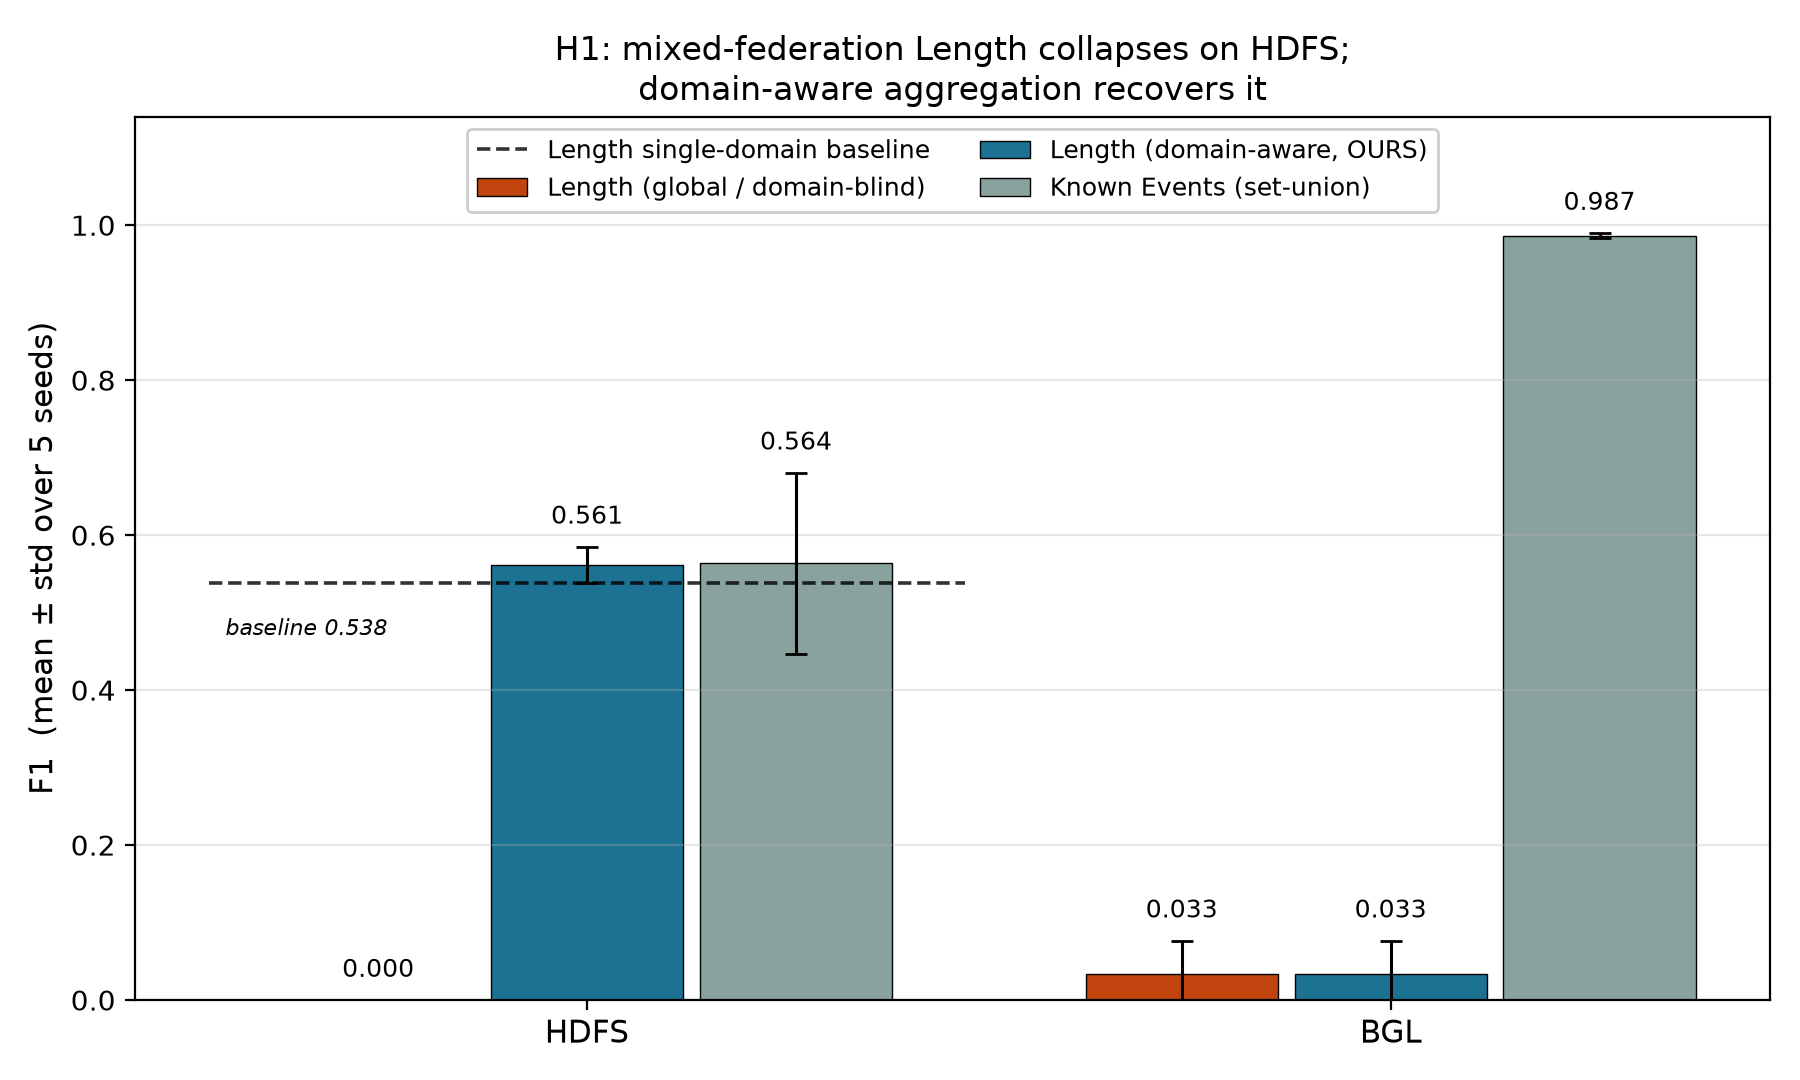
\includegraphics[width=\columnwidth]{h1_collapse_recover.png}
\caption{H1: in the mixed federation, domain-blind Length collapses on HDFS ($F_1\approx0$);
domain-aware aggregation recovers it to the single-domain baseline (dashed). Known Events is
unaffected, and BGL is unchanged by the fix---the contamination and its repair are asymmetric.}
\label{fig:h1}
\end{figure}

\section{H2: Simultaneous Mixed FedAvg Does Not Degrade DeepLog}\label{sec:h2}
Table~\ref{tab:h2} compares single-domain and mixed DeepLog per domain, averaged over three seeds.
The drop is essentially zero on HDFS ($+0.0002\pm0.0001$) and consistently \emph{negative}
(i.e., mixed is better) on BGL ($-0.1058\pm0.0023$). Simultaneous mixed FedAvg thus does not degrade
the deep model; this strengthens, rather than contradicts, the generality of deep federated
detection reported by prior work. With the reference's scalar-id input, HDFS ids occupy $[0,32]$ and
BGL ids $[33,426]$ (disjoint numeric ranges), so the LSTM can separate the domains by input
magnitude alone, and weight averaging never has to reconcile conflicting behaviours on the same
inputs. The negative persists even under a learned embedding (HDFS drop
$-0.0025\pm0.0018$; Section~\ref{sec:mech}), because every FedAvg round sees both domains and the
averaged model maintains both. This robustness, however, does not extend to sequential arrival.

\begin{table}[t]
\caption{H2: DeepLog per-domain $F_1$, single-domain vs.\ mixed (mean $\pm$ std, $n=3$ seeds).
Source: \texttt{results/h2\_multiseed.csv}.}
\label{tab:h2}
\centering
\begin{tabular}{@{}lccc@{}}
\toprule
Domain & Single-domain & Mixed & Drop (single $-$ mixed) \\
\midrule
HDFS & 0.7039 & 0.7037 & $+0.0002\pm0.0001$ \\
BGL  & 0.6459 & 0.7517 & $-0.1058\pm0.0023$ \\
\bottomrule
\end{tabular}
\end{table}

\section{H3: Sequential Arrival---Grow-Forever versus Forget}\label{sec:h3}
Under sequential arrival (HDFS first, then BGL), the two families fail in complementary ways
(Table~\ref{tab:h3}, Fig.~\ref{fig:h3}). Known Events \emph{never forgets} (union is monotone, so
HDFS $F_1$ is unchanged at $0.7885$), but its state grows $\times3.7$ ($1{,}688\rightarrow6{,}300$
bytes) as BGL's vocabulary is absorbed; on an open stream of domains this growth is unbounded,
contradicting C2 under evolution. DeepLog with the scalar-id input shows \emph{no} forgetting (HDFS
$F_1$ unchanged), for the same disjoint-range reason as H2: continued training on BGL updates the
$[33,426]$ input region and barely perturbs the $[0,32]$ region HDFS occupies.

\begin{table}[t]
\caption{H3: sequential arrival (HDFS$\rightarrow$BGL). Forgetting $=F_1$ before $-$ after.
The Known Events and DeepLog (scalar id) rows are single-seed (seed 0) and deterministic; the
DeepLog (embedding) row reports the 3-seed mean $\pm$ std.
Source: \texttt{results/h3\_sequential\{,\_embedding\}.csv}, \texttt{mechanism\_multiseed.csv}.}
\label{tab:h3}
\centering
\begin{tabular}{@{}lccc@{}}
\toprule
Method / input & After HDFS & After BGL & Forgetting \\
\midrule
Known Events         & 0.7885 & 0.7885 & 0.0000 \\
DeepLog (scalar id)  & 0.7037 & 0.7037 & 0.0000 \\
DeepLog (embedding)  & 0.7037 & \textbf{0.039} & $\mathbf{+0.6647 \pm 0.0032}$ \\
\bottomrule
\end{tabular}
\end{table}

\begin{figure}[t]
\centering
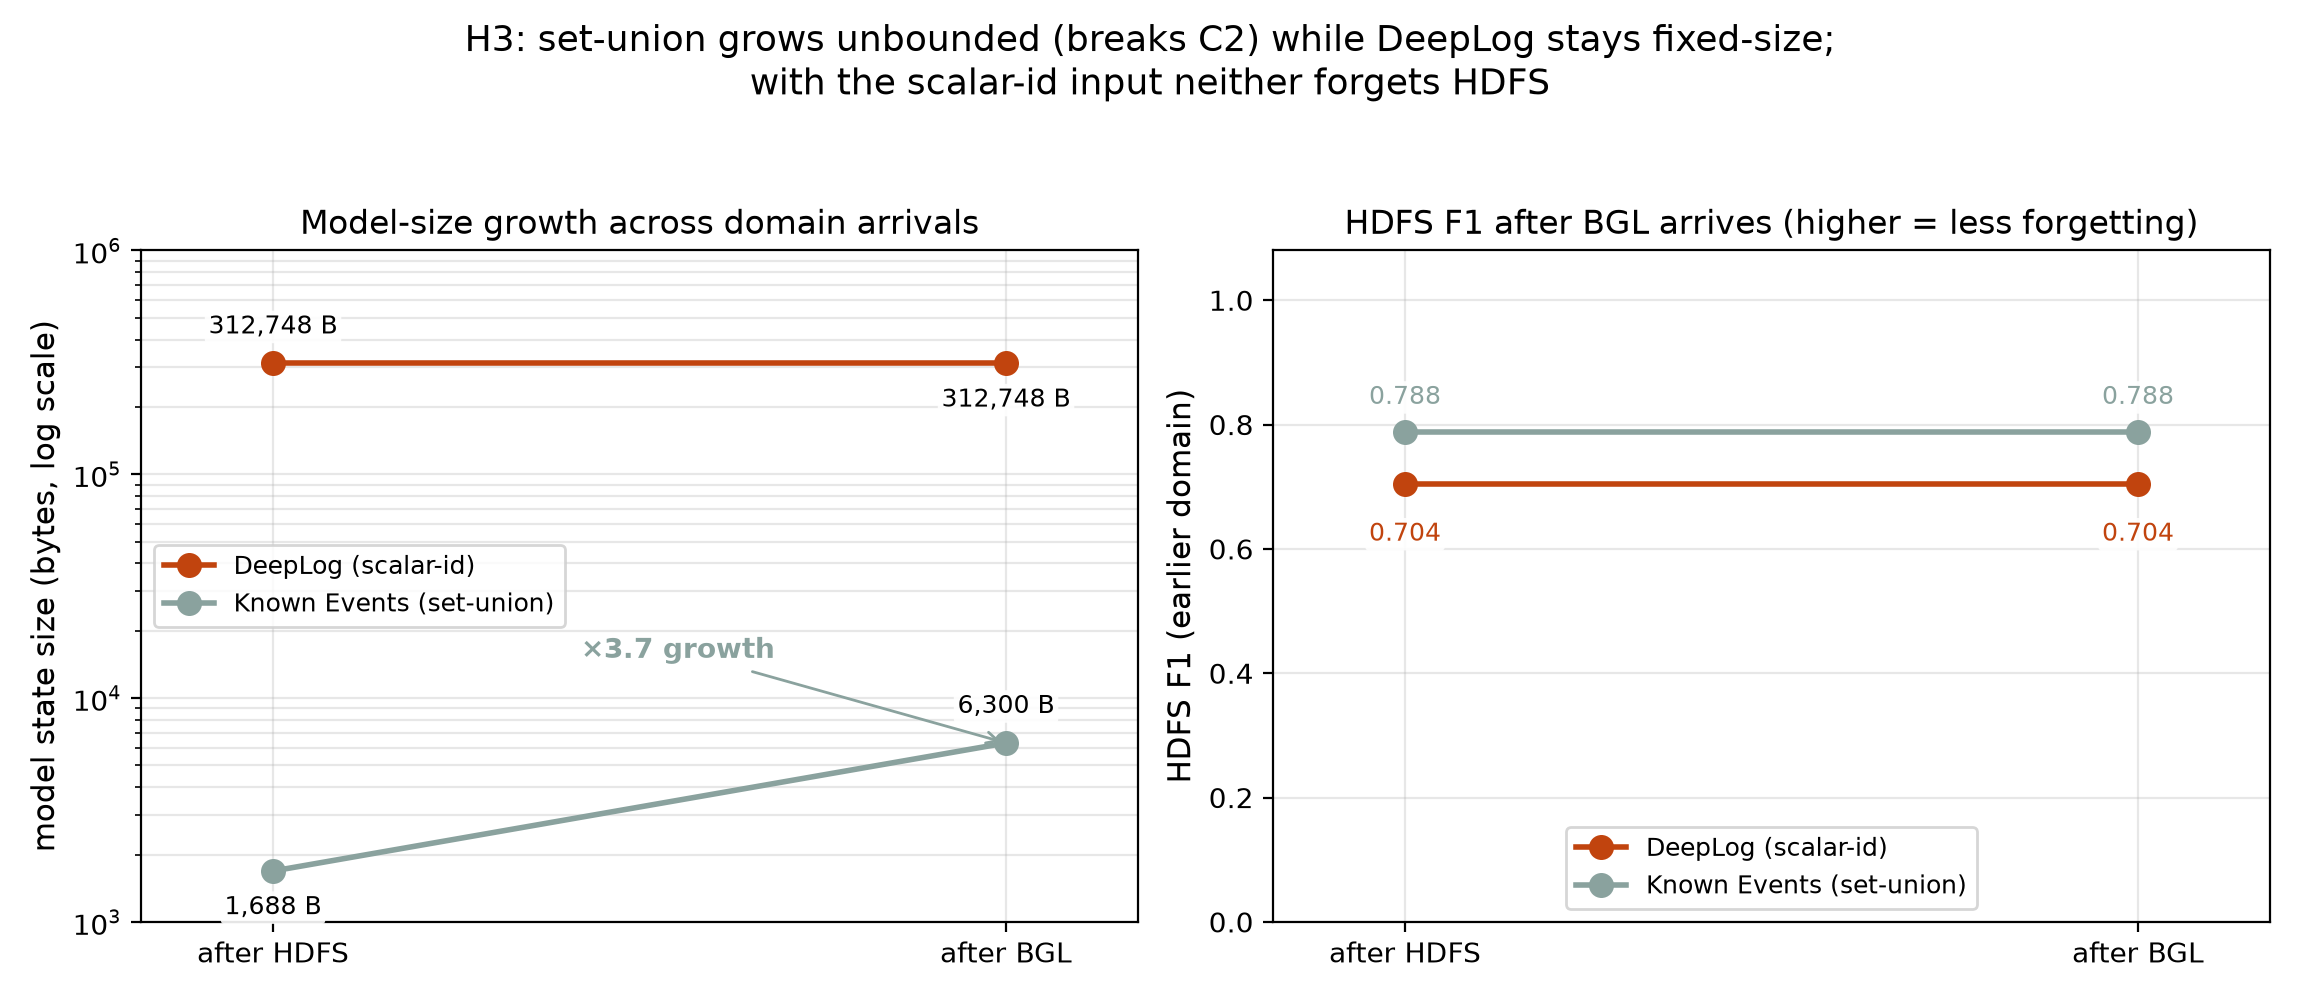
\includegraphics[width=\columnwidth]{h3_sequential.png}
\caption{H3: across domain arrivals, the set-union model grows (left; $\times3.7$) while DeepLog
stays fixed-size; with the scalar-id input neither forgets HDFS (right).}
\label{fig:h3}
\end{figure}

\section{Mechanism: Representation Decides Forgetting}\label{sec:mech}
The H2/H3 negatives above all share one candidate cause: the scalar-id encoding keeps the two
vocabularies in disjoint input ranges. We test this directly by swapping DeepLog's scalar input for
a learned 16-dimensional embedding, where the vocabularies overlap in feature space, and re-running
H2 and H3 over three seeds (Fig.~\ref{fig:mech}). The result is decisive. Under \emph{sequential}
arrival the embedding model \emph{catastrophically forgets} HDFS: forgetting $0.665\pm0.003$, with
HDFS $F_1$ falling from $0.70$ to $0.04$, versus $0.000$ with the scalar input. Under
\emph{simultaneous} mixing the embedding model still does not degrade (HDFS drop
$-0.0025\pm0.0018$). Thus the representation, not the aggregation method, decides whether the deep
model forgets.

The unifying picture is a $2\times2$ over
\{simultaneous mixing, sequential arrival\}$\times$\{disjoint-range input, shared-representation
input\} (Fig.~\ref{fig:map}): only \emph{(sequential, shared representation)} fails, and it fails hard. Simultaneous
mixing is safe; it is sequential onboarding of a domain into a shared-representation model that is
dangerous. This distinction, absent from prior work, explains why the reference's scalar-id
DeepLog appears robust, and predicts that any semantics-based encoding (embeddings, template
vectors, or LLM features), which necessarily shares feature space across domains, will require an
explicit continual-learning defense~\cite{kirkpatrick2017overcoming,delange2022continual}.

\textbf{Forgetting is directional.} A natural follow-up is whether the catastrophic cell is
symmetric in arrival order. We reverse it---BGL first, then HDFS---and measure how much the earlier
domain (now BGL) is retained, over three seeds (Table~\ref{tab:reverse}). It is \emph{not} symmetric:
in the reverse order the embedding model does \emph{not} forget BGL---BGL $F_1$ actually rises from
$0.649$ to $0.752$ (``forgetting'' $-0.103\pm0.006$), and the scalar input is likewise safe
($-0.125\pm0.017$). So the failure is not merely \emph{(sequential, shared representation)} but
specifically \emph{onboarding the broad-vocabulary domain (BGL, 394 events) after the narrow one
(HDFS, 33 events)}: the larger new domain's training dominates the shared representation and overwrites
the narrow region the earlier domain occupied, whereas the reverse---a small vocabulary arriving into a
model that already spans a broad one---perturbs it little. This sharpens the map's failing cell into a
concrete, testable direction rather than weakening it, and it warns that onboarding order is itself a
deployment lever: where possible, introduce broad-vocabulary domains \emph{earlier}.

\begin{table}[t]
\caption{Arrival order is not symmetric. Reverse order (BGL$\rightarrow$HDFS) does not forget the
earlier domain under either input; contrast the forward embedding case (HDFS$\rightarrow$BGL) that
forgets $+0.665$. Mean $\pm$ std, $n=3$ seeds. Source: \texttt{results/h3\_reverse\_order.csv}.}
\label{tab:reverse}
\centering
\begin{tabular}{@{}lccc@{}}
\toprule
Order / input & Earlier before & Earlier after & Forgetting \\
\midrule
HDFS$\rightarrow$BGL, embedding & 0.704 & $0.039\pm0.003$ & $+0.665\pm0.003$ \\
BGL$\rightarrow$HDFS, embedding & 0.649 & $0.752\pm0.000$ & $-0.103\pm0.006$ \\
BGL$\rightarrow$HDFS, scalar id & 0.627 & $0.752\pm0.000$ & $-0.125\pm0.017$ \\
\bottomrule
\end{tabular}
\end{table}

\begin{figure}[t]
\centering
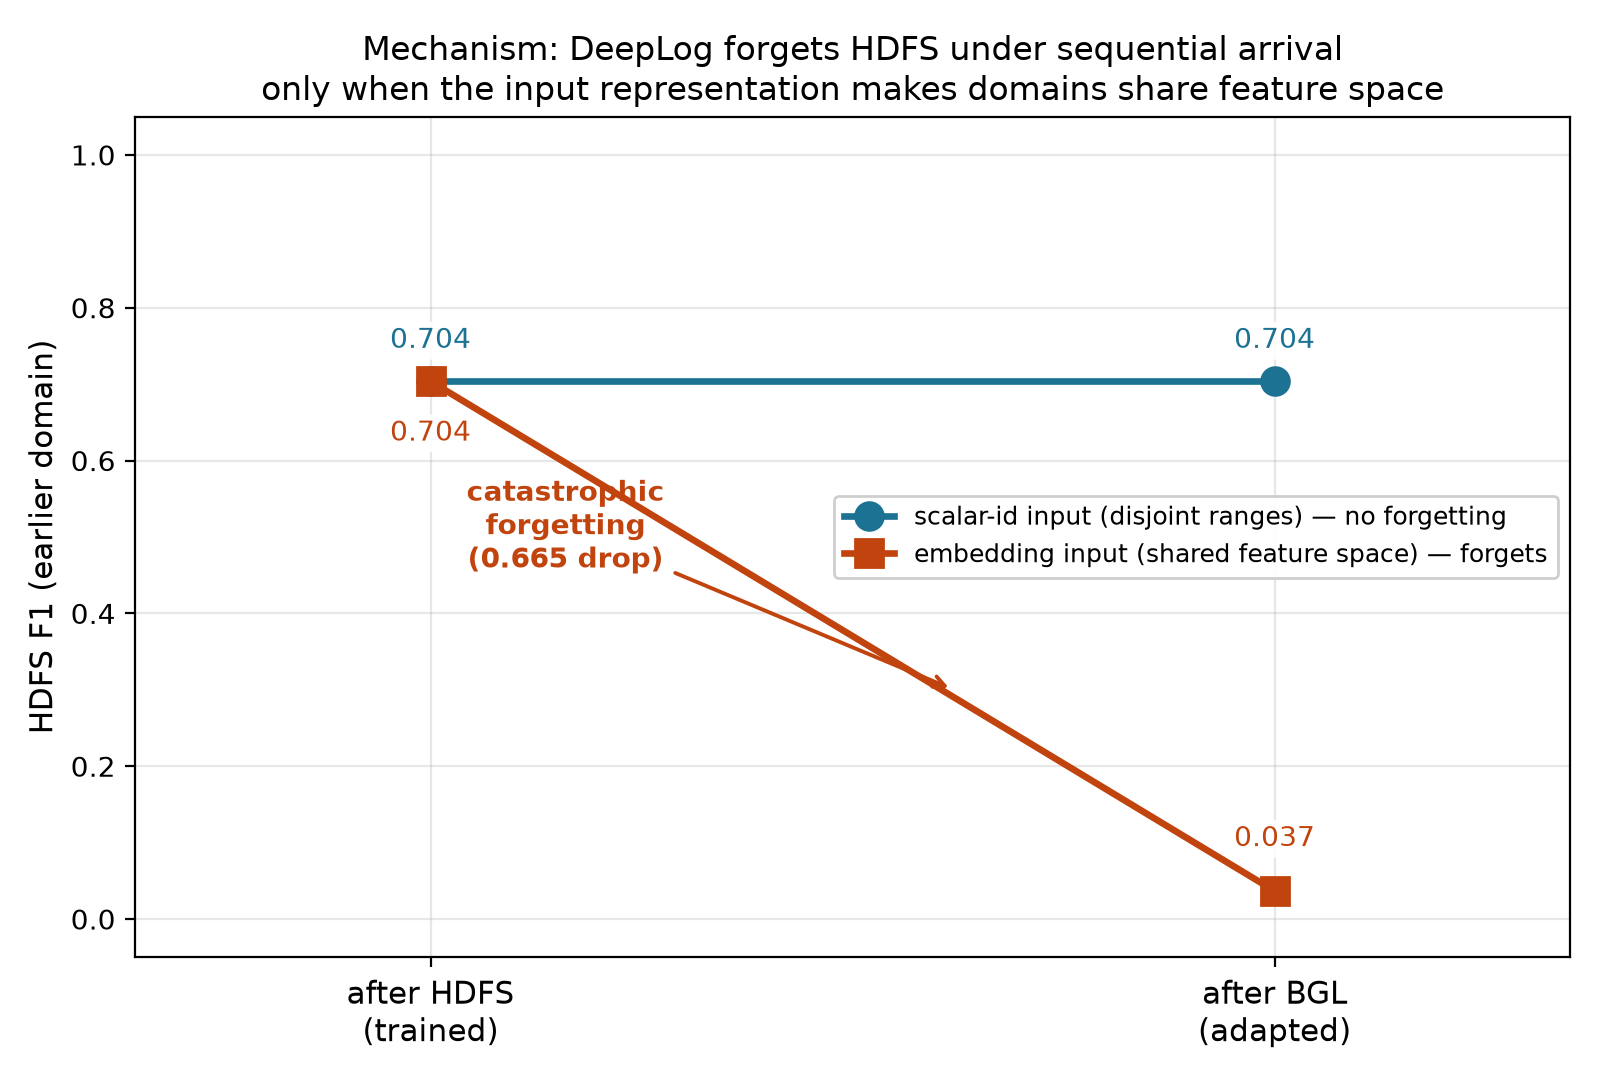
\includegraphics[width=\columnwidth]{mechanism_forgetting.png}
\caption{Mechanism: DeepLog forgets the earlier domain under sequential arrival only when the input
representation makes domains share a feature space (embedding, orange: $0.70\!\rightarrow\!0.04$);
the scalar-id encoding (blue) keeps them in disjoint ranges and no forgetting occurs.}
\label{fig:mech}
\end{figure}

\begin{figure}[t]
\centering
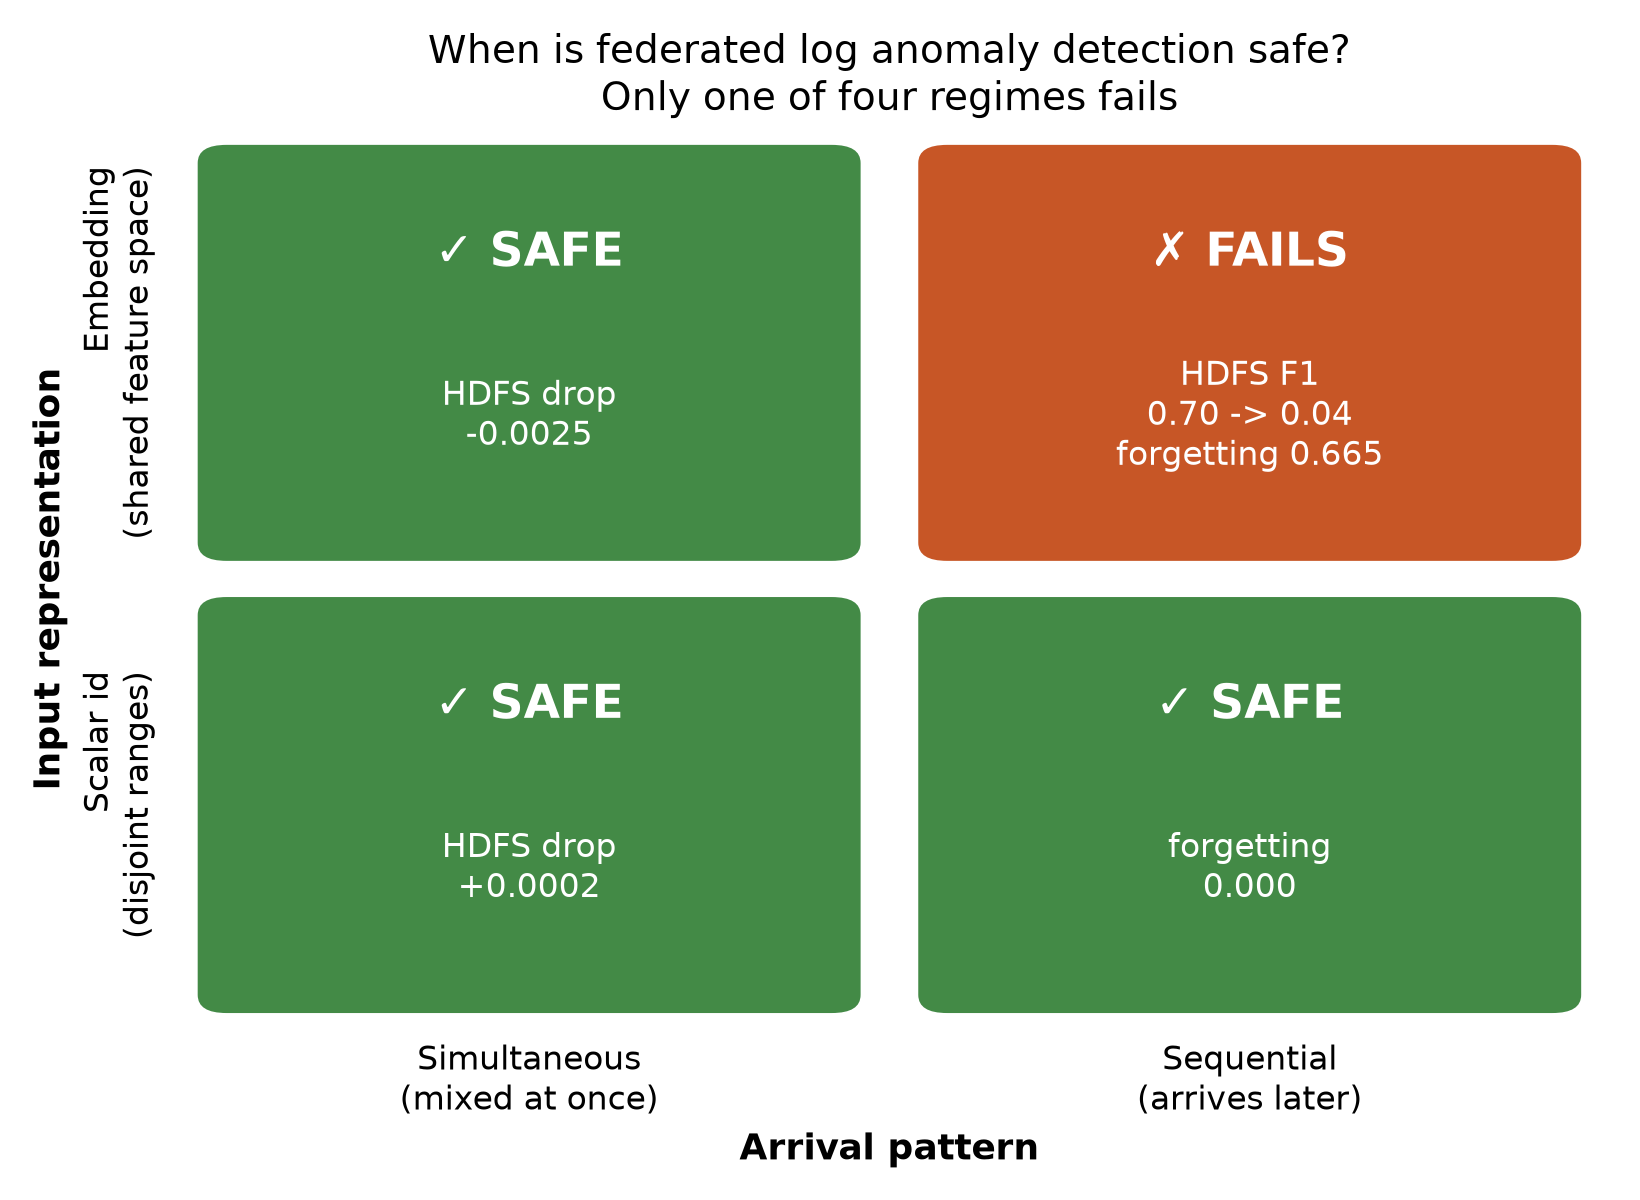
\includegraphics[width=\columnwidth]{two_by_two_map.png}
\caption{The $2\times2$ safety map summarizing H2, H3, and the mechanism experiment. Across
\{arrival pattern\}$\times$\{input representation\}, only \emph{(sequential, shared representation)}
fails; the other three regimes are safe. Values are the measured per-domain drop or forgetting. The
failing cell is shown for the forward order HDFS$\rightarrow$BGL; it is directional (Table~\ref{tab:reverse}).}
\label{fig:map}
\end{figure}

\section{Mitigation: Replay Restores the Forgotten Domain}\label{sec:replay}
The mechanism above identifies \emph{(sequential arrival, shared representation)} as the single
failing cell; a diagnosis is only actionable if the failure is fixable. We test the simplest
continual-learning defense---experience replay~\cite{delange2022continual}: when the new domain (BGL)
arrives, we retain a small buffer of the earlier domain's (HDFS) training sequences and train on
BGL and the buffer jointly, as one extra federated client, instead of on BGL alone. The buffer is a
$p$-fraction sample of the pooled HDFS training set ($5{,}582$ sequences, itself the reference's
$1\%$ regime); everything else---embedding input, rounds, seeds---is unchanged from
Section~\ref{sec:mech}. Because replay stores raw sequences and not parameters, the model remains
fixed-size.

Table~\ref{tab:replay} and Fig.~\ref{fig:replay} report the result over three seeds. Without replay
the embedding model forgets HDFS ($F_1$ $0.70\!\rightarrow\!0.04$, forgetting $0.665\pm0.003$, reproducing
Section~\ref{sec:mech}). A buffer of just $10\%$ ($\approx558$ sequences) \emph{eliminates}
forgetting---HDFS returns to $0.700\pm0.004$, its pre-arrival level---while BGL is still learned
($0.722\pm0.052$), and a $25\%$ buffer is cleaner still (forgetting $0.001\pm0.001$, BGL
$0.758\pm0.009$). A $5\%$ buffer is too small to be reliable (it recovers HDFS in only one of three
seeds, giving forgetting $0.440\pm0.308$), which delimits how small the buffer can be. The failure
the paper identifies is therefore real but remediable at negligible cost: a few hundred stored
sequences, no architecture change, and no loss on the new domain. This makes the practitioner
guidance concrete---if sequential onboarding into a shared-representation model is unavoidable,
budget a small replay buffer.

\subsection{A memory-free alternative: EWC}\label{sec:ewc}
Replay stores raw sequences of the earlier domain, which some deployments cannot do (data-retention
limits, or a client that has left the federation). We therefore also evaluate the standard
\emph{parameter-based}, memory-free defense---elastic weight consolidation
(EWC)~\cite{kirkpatrick2017overcoming}---under the identical protocol. From the stage-1 HDFS model we
estimate the empirical Fisher information $F_i$ of each weight on HDFS windows, then continue federated
training on BGL with the penalty $(\lambda/2)\sum_i F_i(\theta_i-\theta_i^\ast)^2$ anchoring the
HDFS-important weights $\theta^\ast$. Table~\ref{tab:ewc} sweeps $\lambda$ over three seeds. EWC
\emph{does} remove the forgetting---at $\lambda{=}10^{8}$ it restores HDFS to $0.690\pm0.005$
(forgetting $0.014\pm0.005$) while BGL is still learned ($0.752\pm0.052$), matching replay's outcome
without storing any data. The catch is tuning: the penalty has no effect until $\lambda{=}10^{6}$ and
only succeeds at $\lambda{=}10^{8}$, i.e.\ EWC must be tuned across six orders of magnitude, whereas
replay works out of the box at a $10\%$ buffer. The practical takeaway is a genuine trade-off rather
than a single winner: prefer replay when a small earlier-domain buffer is permissible (no tuning),
and EWC when it is not (no storage, but a sensitive hyper-parameter to calibrate).

\begin{table}[t]
\caption{Memory-free EWC for embedding-DeepLog under sequential arrival (HDFS$\rightarrow$BGL),
mean $\pm$ std over $n=3$ seeds. EWC removes the forgetting only at $\lambda{=}10^{8}$; smaller
$\lambda$ barely helps. Source: \texttt{results/mitigation\_ewc.csv}.}
\label{tab:ewc}
\centering
\begin{tabular}{@{}lccc@{}}
\toprule
EWC $\lambda$ & HDFS $F_1$ after & BGL $F_1$ after & Forgetting \\
\midrule
$0$ (no defense) & $0.039\pm0.003$ & $0.642\pm0.028$ & $+0.665\pm0.003$ \\
$10^{2}$         & $0.040\pm0.004$ & $0.649\pm0.019$ & $+0.664\pm0.004$ \\
$10^{4}$         & $0.044\pm0.010$ & $0.651\pm0.015$ & $+0.659\pm0.010$ \\
$10^{6}$         & $0.212\pm0.174$ & $0.663\pm0.047$ & $+0.491\pm0.174$ \\
$10^{8}$         & $\mathbf{0.690\pm0.005}$ & $0.752\pm0.052$ & $\mathbf{+0.014\pm0.005}$ \\
\bottomrule
\end{tabular}
\end{table}

\begin{table}[t]
\caption{Replay mitigation for embedding-DeepLog under sequential arrival (HDFS$\rightarrow$BGL),
mean $\pm$ std over $n=3$ seeds. Buffer $=p\times$ the $5{,}582$-sequence HDFS training pool.
A $\ge10\%$ buffer restores HDFS to its pre-arrival $F_1$ ($0.704$) while BGL is still learned.
Source: \texttt{results/mitigation\_replay.csv}.}
\label{tab:replay}
\centering
\begin{tabular}{@{}lccc@{}}
\toprule
Buffer & HDFS $F_1$ after & BGL $F_1$ after & Forgetting \\
\midrule
none (reproduce)   & $0.039\pm0.003$ & $0.642\pm0.028$ & $+0.665\pm0.003$ \\
$5\%$ (279 seq)    & $0.264\pm0.308$ & $0.651\pm0.002$ & $+0.440\pm0.308$ \\
$10\%$ (558 seq)   & $\mathbf{0.700\pm0.004}$ & $0.722\pm0.052$ & $\mathbf{+0.004\pm0.004}$ \\
$25\%$ (1396 seq)  & $0.702\pm0.001$ & $0.758\pm0.009$ & $+0.001\pm0.001$ \\
$50\%$ (2791 seq)  & $0.694\pm0.014$ & $0.752\pm0.000$ & $+0.009\pm0.014$ \\
\bottomrule
\end{tabular}
\end{table}

\begin{figure}[t]
\centering
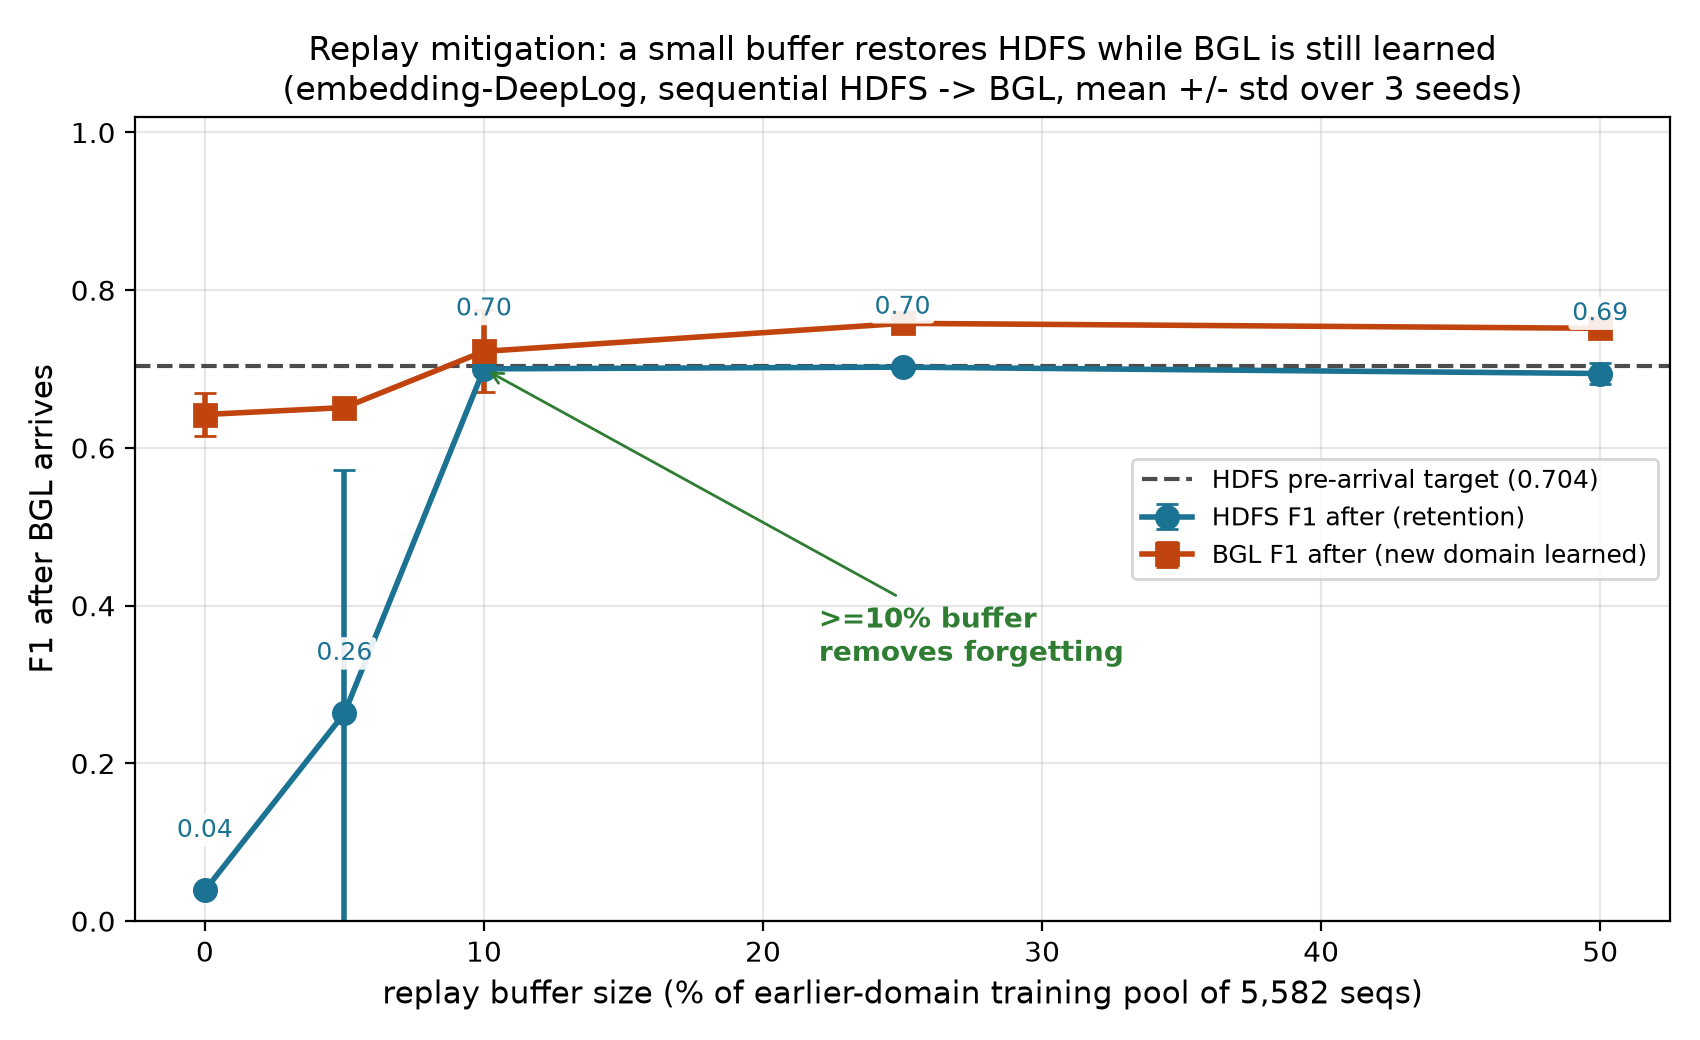
\includegraphics[width=\columnwidth]{replay_mitigation.png}
\caption{Replay mitigation: HDFS retention and BGL learning versus buffer size (mean $\pm$ std,
three seeds). Without a buffer HDFS collapses to $0.04$; a $\ge10\%$ buffer restores it to its
pre-arrival level (dashed) while BGL is still learned. The $5\%$ point is unreliable (large
variance), which delimits the minimum useful buffer.}
\label{fig:replay}
\end{figure}

\section{Does the Fix Lift the Full Ensemble?}\label{sec:ensemble}
The reference's strongest HDFS method is the union ensemble Events\,$\lor$\,Length\,$\lor$\,ECVC.
We first reproduce it: the single-domain HDFS ensemble reaches $F_1=0.984$ (the reference reports
$\sim$0.95). In the mixed federation (Table~\ref{tab:ens}), swapping domain-blind for domain-aware
Length leaves the ensemble $F_1$ \emph{unchanged}. The reason is structural: the combination is a
logical OR, so a collapsed Length cannot lower recall, and on HDFS ECVC alone already reaches
$F_1=0.968$ (recall $0.96$), driving the union's recall to $\approx1.0$. A recovered Length only
adds detections the ensemble already makes.
We therefore \emph{scope} H1's practical impact honestly: domain-aware aggregation is decisive for
\emph{lightweight-only} deployments (Length/Events without a costly nearest-neighbour store, exactly
the efficiency regime~\cite{pustozerova2026lightweight} motivates), where HDFS Length moves from
$0.000$ to $0.561$; it does not change the full ensemble, which is carried by ECVC. We do not claim
domain mixing breaks the reference's best method.

\begin{table}[t]
\caption{Ensemble Events\,$\lor$\,Length\,$\lor$\,ECVC: HDFS $F_1$ is unchanged by the Length fix
because ECVC dominates the union. Source: \texttt{results/ensemble.csv}.}
\label{tab:ens}
\centering
\begin{tabular}{@{}lc@{}}
\toprule
HDFS ensemble & $F_1$ \\
\midrule
Single-domain (reference target) & 0.9836 \\
Mixed, Length global (collapsed 0.0002) & 0.9837 \\
Mixed, Length domain-aware (recovered 0.5379) & 0.9836 \\
\bottomrule
\end{tabular}
\end{table}

\section{Discussion}
Our results refine the two published claims rather than overturn them wholesale. C1 (invariance)
\emph{fails} for range-based aggregation under domain skew, and a per-domain fix restores it; it
survives for set-union. C2 (bounded growth) \emph{fails} for set-union under sequential arrival
(unbounded vocabulary growth) while the deep model stays fixed-size. For the deep model, the
practically important axis is not mixing but \emph{arrival pattern combined with representation}:
simultaneous FedAvg is safe, but sequential onboarding into a shared-representation model forgets
catastrophically. For practitioners this yields concrete guidance: (i) use per-domain parameters for
any range/threshold statistic in a heterogeneous federation; (ii) prefer simultaneous over sequential
onboarding when possible; and (iii) if sequential onboarding is unavoidable with a semantics-based
model, budget a small replay buffer, which we show (Section~\ref{sec:replay}) removes the forgetting
at the cost of a few hundred stored sequences and no architecture change.

\section{Threats to Validity}
\textbf{DeepLog absolute level.} Our single-domain HDFS DeepLog operates at $F_1\approx0.70$
(best $0.7205$ over a $1$--$100$ round sweep; \texttt{results/deeplog\_convergence\_*}), not the
reference's headline $\sim$0.91--0.93. Neither additional training nor tuning the top-$g$ threshold
reaches $0.93$: $F_1$ plateaus by round 5, and recall is hard-capped at $\sim$0.63 for every $g$
(\texttt{results/deeplog\_num\_candidates\_sweep.csv}), meaning roughly a third of HDFS anomalies are
predicted perfectly by the next-event model and are unrecoverable by any threshold. The reference's
\emph{federated} configuration itself trains only one round of one epoch on $1\%$ of normals, so our
value is consistent with its federated regime; the $\sim$0.93 figure is most plausibly the
reference's centralized or best-tuned result. To test the capacity ceiling directly, we ran a
standalone \emph{centralized} DeepLog on the \emph{full} HDFS normal set (all $558{,}223$ sequences,
$6.67$M training windows, no federation; \texttt{results/deeplog\_centralized\_hdfs.csv}). The run was
budgeted for up to $100$ passes but had fully converged by round ${\sim}30$ and was stopped at $55$.
It likewise does not approach $0.93$: training loss plateaus at $\approx0.204$ by round $20$
(and drifts only to $0.203$ by round $55$), and the transductive $F_1$ peaks at $0.43$ (round $2$)
before settling near $0.25$ (mean $0.257\pm0.016$ over rounds $10$--$55$), with precision saturating
at $\approx0.98$ while recall never exceeds $0.29$. This confirms the ceiling is a property of the scalar-input
next-event model and the top-$g$ rule, not an artifact of federation or of $1\%$ subsampling. We
therefore do not claim to reproduce $0.93$, and all H2/H3 DeepLog numbers are the federated-$1\%$-data
regime. Importantly, the H3 forgetting finding is a
\emph{relative} effect ($0.70\!\rightarrow\!0.04$ under embedding vs.\ $0.70\!\rightarrow\!0.70$ under
scalar), and does not depend on the absolute level; H2 and H3 were run at 12 rounds, already at the
plateau.

\textbf{Other threats.} We use two domains (HDFS, BGL); two genuinely different domains already
exhibit the failure, and more would widen the predicted gap, but generalization to further domains
(e.g., Thunderbird, Spirit) is future work requiring new parsers. Known Events shows high seed
variance on HDFS ($0.56\pm0.12$), which we report openly. Our DeepLog evaluation treats sequences
shorter than the window as normal; because the single-vs-mixed comparison uses an identical harness,
the relative effect is unaffected. ECVC uses a transductive (test-set) threshold, following the
reference convention. Finally, like~\cite{pustozerova2026lightweight}, we compare only within our own
controlled codebase with averaged runs and do not make cross-study metric comparisons.

\section{Conclusion and Future Work}
We tested whether two reported properties of federated log anomaly detection survive a heterogeneous
and evolving federation. Range-based aggregation collapses under domain mixing, and a minimal
domain-aware aggregation restores it to single-domain performance. Simultaneous mixed FedAvg on the
deep model is robust, but sequential onboarding into a shared-representation model forgets
catastrophically (a danger the reference's scalar-id encoding happens to mask), while set-union
detectors never forget but grow unbounded. The contribution is a reproducible account of how the
failure depends jointly on the detection method, the arrival pattern, the input representation, and the
onboarding \emph{direction}, together with working fixes for both failing cases: a domain-aware
aggregation that routes without an oracle tag, and---for the forgetting---both a small replay buffer and
a memory-free EWC penalty, which we compare directly. Future work includes (i) longer arrival sequences
($>2$ domains), where replay-buffer sizing, EWC $\lambda$ scheduling, and cross-domain interference
compound; (ii) additional log domains (e.g., Thunderbird, Spirit) to stress the map beyond the two-domain
containment condition; and (iii) automatic selection of the EWC penalty, whose six-order-of-magnitude
sensitivity we document as its main practical drawback relative to replay.

% -------------------------------------------------------------------------------------
% References are embedded inline so the paper renders without a BibTeX pass.
% A BibTeX-based bibliography is also available: to use it, delete the thebibliography
% block below and uncomment the two lines here. (references.bib holds the same entries.)
% \bibliographystyle{IEEEtran}
% \bibliography{references}
% Entries are ordered by first citation, IEEE style.
% -------------------------------------------------------------------------------------
\begin{thebibliography}{99}

\bibitem{he2016experience}
S.~He, J.~Zhu, P.~He, and M.~R.~Lyu, ``Experience report: System log analysis for anomaly
detection,'' in \emph{Proc. IEEE 27th Int. Symp. Softw. Rel. Eng. (ISSRE)}, 2016, pp.~207--218.

\bibitem{landauer2023survey}
M.~Landauer, S.~Onder, F.~Skopik, and M.~Wurzenberger, ``Deep learning for anomaly detection
in log data: A survey,'' \emph{Mach. Learn. Appl.}, vol.~12, p.~100470, 2023.

\bibitem{mcmahan2017communication}
B.~McMahan, E.~Moore, D.~Ramage, S.~Hampson, and B.~Ag\"{u}era y Arcas,
``Communication-efficient learning of deep networks from decentralized data,'' in
\emph{Proc. 20th Int. Conf. Artif. Intell. Statist. (AISTATS)}, 2017, pp.~1273--1282.

\bibitem{pustozerova2026lightweight}
A.~Pustozerova, A.~Garc\'{i}a G\'{o}mez, M.~Landauer, M.~Wurzenberger, F.~Skopik, E.~Weippl,
R.~Mayer, and A.~Ekelhart, ``Lightweight techniques for federated anomaly detection in log
data,'' \emph{IEEE Trans. Rel.}, vol.~75, 2026, doi: 10.1109/TR.2026.3677674.

\bibitem{du2017deeplog}
M.~Du, F.~Li, G.~Zheng, and V.~Srikumar, ``DeepLog: Anomaly detection and diagnosis from system
logs through deep learning,'' in \emph{Proc. ACM SIGSAC Conf. Comput. Commun. Secur. (CCS)},
2017, pp.~1285--1298.

\bibitem{meng2019loganomaly}
W.~Meng \emph{et al.}, ``LogAnomaly: Unsupervised detection of sequential and quantitative
anomalies in unstructured logs,'' in \emph{Proc. 28th Int. Joint Conf. Artif. Intell. (IJCAI)},
2019, pp.~4739--4745.

\bibitem{he2017drain}
P.~He, J.~Zhu, Z.~Zheng, and M.~R.~Lyu, ``Drain: An online log parsing approach with fixed depth
tree,'' in \emph{Proc. IEEE Int. Conf. Web Services (ICWS)}, 2017, pp.~33--40.

\bibitem{zhu2023loghub}
J.~Zhu, S.~He, P.~He, J.~Liu, and M.~R.~Lyu, ``Loghub: A large collection of system log datasets
for AI-driven log analytics,'' in \emph{Proc. IEEE 34th Int. Symp. Softw. Rel. Eng. (ISSRE)},
2023. (arXiv:2008.06448.)

\bibitem{zhao2018federated}
Y.~Zhao, M.~Li, L.~Lai, N.~Suda, D.~Civin, and V.~Chandra, ``Federated learning with non-IID
data,'' \emph{arXiv preprint arXiv:1806.00582}, 2018.

\bibitem{kairouz2021advances}
P.~Kairouz, H.~B.~McMahan, B.~Avent \emph{et al.}, ``Advances and open problems in federated
learning,'' \emph{Found. Trends Mach. Learn.}, vol.~14, no.~1--2, pp.~1--210, 2021.

\bibitem{fedlog2024openchallenges}
P.~Himler, M.~Landauer, F.~Skopik, and M.~Wurzenberger, ``Anomaly detection in log-event
sequences: A federated deep learning approach and open challenges,'' \emph{Mach. Learn. Appl.},
vol.~16, p.~100554, 2024.

\bibitem{fedlad2025}
Y.~Liao, J.~Keung, Z.~Mao, J.~Zhang, and J.~Li, ``FedLAD: A modular and adaptive testbed for
federated log anomaly detection,'' \emph{arXiv preprint arXiv:2512.08277}, 2025.

\bibitem{kirkpatrick2017overcoming}
J.~Kirkpatrick \emph{et al.}, ``Overcoming catastrophic forgetting in neural networks,''
\emph{Proc. Nat. Acad. Sci. (PNAS)}, vol.~114, no.~13, pp.~3521--3526, 2017.

\bibitem{delange2022continual}
M.~De~Lange, R.~Aljundi, M.~Masana, S.~Parisot, X.~Jia, A.~Leonardis, G.~Slabaugh, and
T.~Tuytelaars, ``A continual learning survey: Defying forgetting in classification tasks,''
\emph{IEEE Trans. Pattern Anal. Mach. Intell.}, vol.~44, no.~7, pp.~3366--3385, 2022.

\bibitem{cfl2023quantifying}
C.~Dupuy, J.~Majmudar, J.~Wang, T.~G.~Roosta, R.~Gupta, C.~Chung, J.~Ding, and S.~Avestimehr,
``Quantifying catastrophic forgetting in continual federated learning,'' in \emph{Proc. IEEE Int.
Conf. Acoust., Speech, Signal Process. (ICASSP)}, 2023, pp.~1--5.

\bibitem{ecvc2024}
M.~Landauer, F.~Skopik, and M.~Wurzenberger, ``A critical review of common log data sets used for
evaluation of sequence-based anomaly detection techniques,'' \emph{Proc. ACM Softw. Eng.},
vol.~1, no.~FSE, pp.~1354--1375, 2024, doi: 10.1145/3660768.

\end{thebibliography}

\end{document}
